\subsection{Comportamento dinamico}

La caratterizzazione dello ShuntLDO a $2 \A$ fin qui discussa \`e limitata al caso stazionario con carichi statici.
\`E per\`o fondamentale studiare il comportamento dello ShuntLDO in risposta a variazioni dinamiche del carico, focalizzando l'attenzione sulla velocità dello ShuntLDO nel reagire alla variazioni di consumo di corrente nel carico. 
La risposta dinamica dipende da molti fattori tra cui il punto di lavoro scelto per ShuntLDO, il scale dei tempi in cui avviene la variazione di carico e l'entità di tale variazione.

Per effettuare queste prove, si è alimentato il circuito tramite un generatore di corrente a $1.5\A$, ponendo la tensione di riferimento a $\mathrm{V_{ref}=0.5 \V}$ per avere una tensione regolata nominale $\VDD=1\V$. %, ci aspettiamo una tensione all'uscita di $1 \V$.
Sulla scheda di test, per emulare un carico dinamico, è presente un mosfet posto in parallelo al carico statico, $\mathrm{R_{load}}$, come visibile nelle Figure~\ref{Setupscheme} e~\ref{TransientTest}, pilotato tramite un opportuno segnale sul gate che definisce durata e entit\`a dell'impulso di corrente addizionale $\mathrm{I_{mosfet}}$ che si somma a quella stazionaria che scorre in $\mathrm{R_{load}}$. Il resistore R5, di $0.1 \Omega$, posto in serie al drain del mosfet \`e utizzato per misurare $\mathrm{I_{mosfet}}$.

Tramite un generatore di segnali connesso al gate del mosfet, si \`e generata una $\mathrm{I_{mosfet}}$ con il profilo temporale di un'onda quadra. L'impulso di carico aggiuntivo ha durata (diversi $\us$) e frequenza (decine di Hz) tali che i transienti consecutivi sono sempre sufficientemente lontani da permettere allo ShuntLDO di raggiungere ogni volta lo stato stazionario. In altre parole si sono studiati indipendentemente gli effetti indotti dal fronte di salita (e di discesa) del carico aggiuntivo con particolare attenzione alle variazioni in ampiezza di $\mathrm{V_{in}}$ e $\mathrm{V_{out}}$, in corrispondenza del transiente di $\mathrm{I_{mosfet}}$, e ai tempi di recupero in funzione di $\mathrm{I_{mosfet}}$ e con $\mathrm{R_{load}}$ fissata.
\begin{figure}[!htb]
\centering
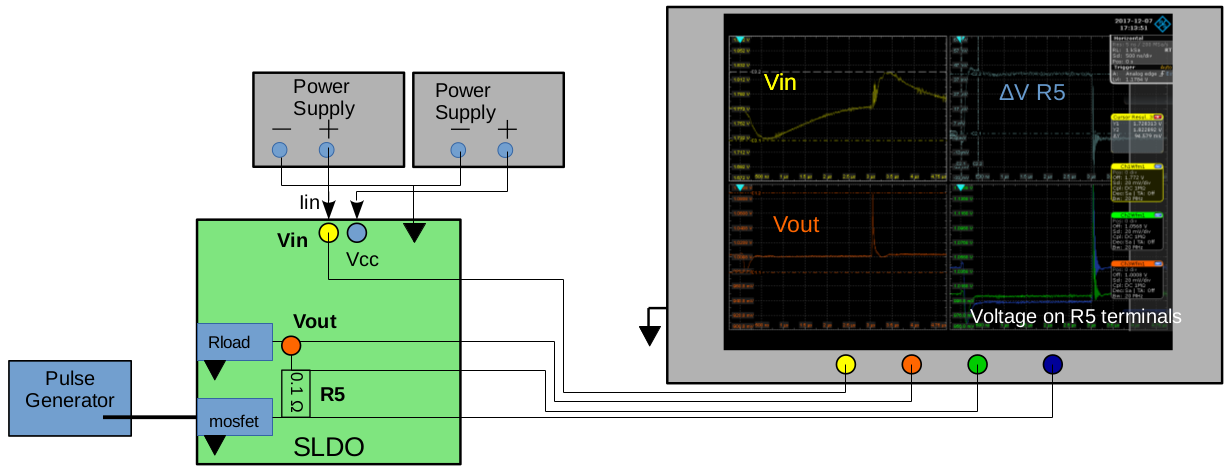
\includegraphics[width=.99\linewidth]{Immagini/SetupScheme}
\caption{Schema dell'allestimento per lo studio del comportamento dinamico dello ShuntLDO. In grigio sono riportati gli alimentatori e in verde è rappresentata la scheda di test su cui, in azzurro, sono evidenziati mosfet e carico resistivo. Collegato al Gate del mosfet, sulla sinistra, vi è l'impulsatore. Sulla destra è rappresentato l'oscilloscopio attraverso cui sono monitorate le tensioni di ingresso $\mathrm{V_{in}}$, di uscita $\mathrm{V_{out}}$ e quelle ai capi di R5. I triangoli color ciano, presenti nella parte alta di ciascun grafico, marcano la posizione temporale del trigger, fornito esternamente, e corrispondente al fronte di salita dell'impulso in ingresso al Gate del mosfet.}
\label{Setupscheme}
\end{figure}

Fin dalle prime misure con l'oscilloscopio si è notato per\`o che l'utilizzo del mosfet come carico dinamico induce contaminazioni sui profili temporali, dovute probabilmente al mosfet stesso pi\`u che al circuito in esame, rendendo difficile l'interpretazione dei risultati.
\begin{figure}
\begin{subfigure}{.5\textwidth}
  \centering
  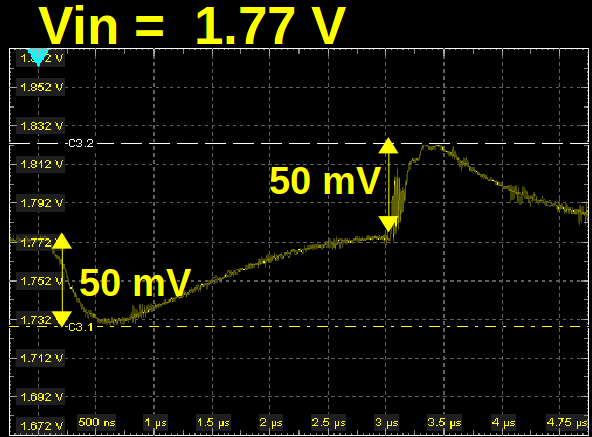
\includegraphics[width=.96\linewidth]{Immagini/zoomTransientTest1}
  \caption{ }
  \label{TransientTest:sfig1}
\end{subfigure}%
\begin{subfigure}{.5\textwidth}
  \centering
  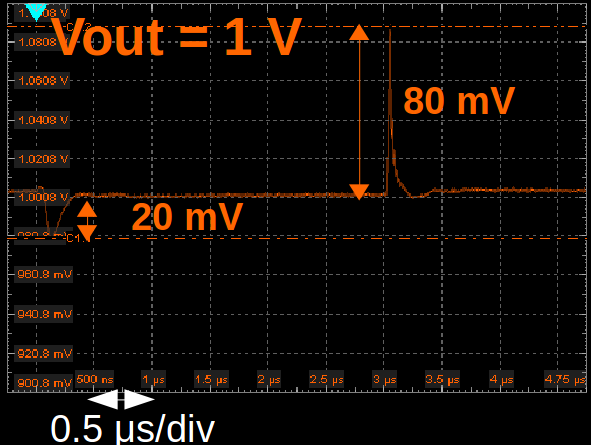
\includegraphics[width=.95\linewidth]{Immagini/zoomTransientTest2}
  \caption{ }
  \label{TransientTest:sfig2}
\end{subfigure}
\begin{subfigure}{\textwidth}
  \centering
  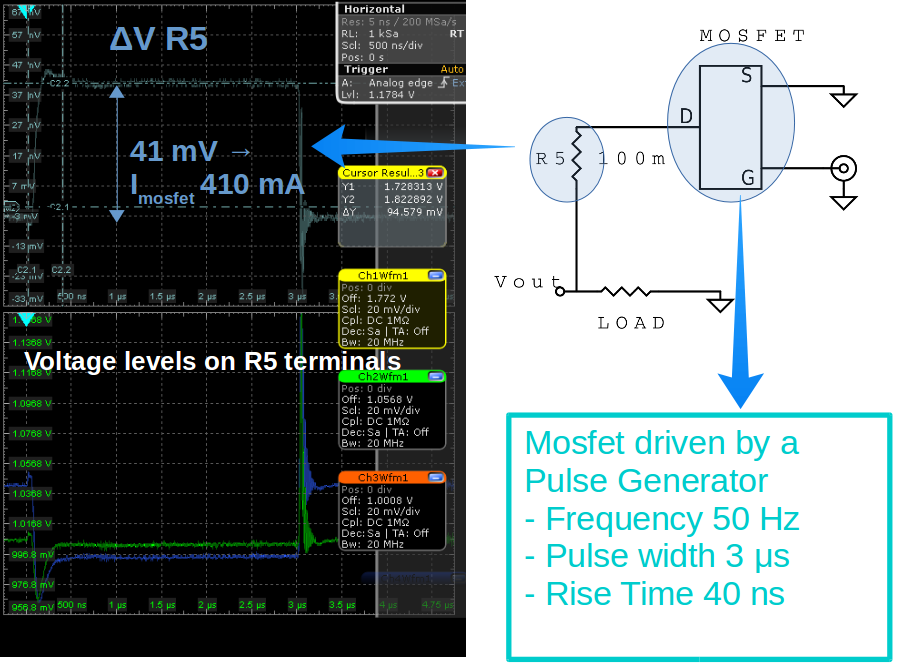
\includegraphics[width=0.95\linewidth]{Immagini/zoomTransientTest3bis}
  \caption{ }
  \label{TransientTest:sfig3}
\end{subfigure}
\caption{Schermate dell'oscilloscopio catturate durante le misure dello ShuntLDO con carico dinamico: in giallo è rappresentata la tensione in ingresso, in arancione quella in uscita e in verde e blu, rispettivamente, la tensione sui i terminali di R5, la cui differenza è riportata in azzurro. In (c), a lato della schermata dell'oscilloscopio, è riportato lo schematico della parte di circuito con mosfet e resistenza. I triangoli color ciano, presenti nella parte alta di ciascun grafico, marcano la posizione temporale del trigger, fornito esternamente e corrispondente al fronte di salita di $\mathrm{I_{mosfet}}$.}
\label{TransientTest}
\end{figure}
Prendendo come riferimento la Fig.~\ref{TransientTest}, si può notare infatti un'asimmetria nelle variazioni di $\mathrm{V_{out}}$, riportato in arancione nel grafico in alto a destra.
Allo stesso modo nella sottofigura~\ref{TransientTest:sfig3} in azzurro, è riportata la differenza tra le tensioni misurate ai capi di R5 (in blu e verde nel grafico in basso) e in cui si osserva un'asimmetria tra il fronte di salita e di discesa di $\mathrm{I_{mosfet}}$, che varia tra 0 e $\sim 400\mA$. In particolare sono visibili delle oscillazioni, sia sulle tensioni riferite a R5 sia sul $\mathrm{V_{out}}$, in corrispondenza del fronte di discesa di $\mathrm{I_{mosfet}}$, ovvero quando il mosfet si spegne.

\subsubsection{Caratterizzazione dell'impulso di corrente di prova}
 
Prima di procedere a misure dinamiche estensive per varie combinazioni $\mathrm{I_{mosfet}}$--$\mathrm{R_{load}}$, si è cercato di determinare l'origine del fenomeno spurio sopra descritto, sospettando che possa dipendere dalle prestazioni nel dominio temporale del mosfet che equipaggia la scheda di test.

% L'impulso utilizzato in questa prima fase ha:
% \begin{itemize}
%   \item frequenza di $50\Hz$;
%   \item durata di 3 $\mu$s;
%   \item fronte di salita di $40 \ns$.
% \end{itemize}
%In questa prima fase l'impulso utilizzato ha le seguenti caratteristiche: frequenza 50 Hz, durata 3 $\mu$s, durata del fronte di salita 40 ns.

\begin{figure}
\centering
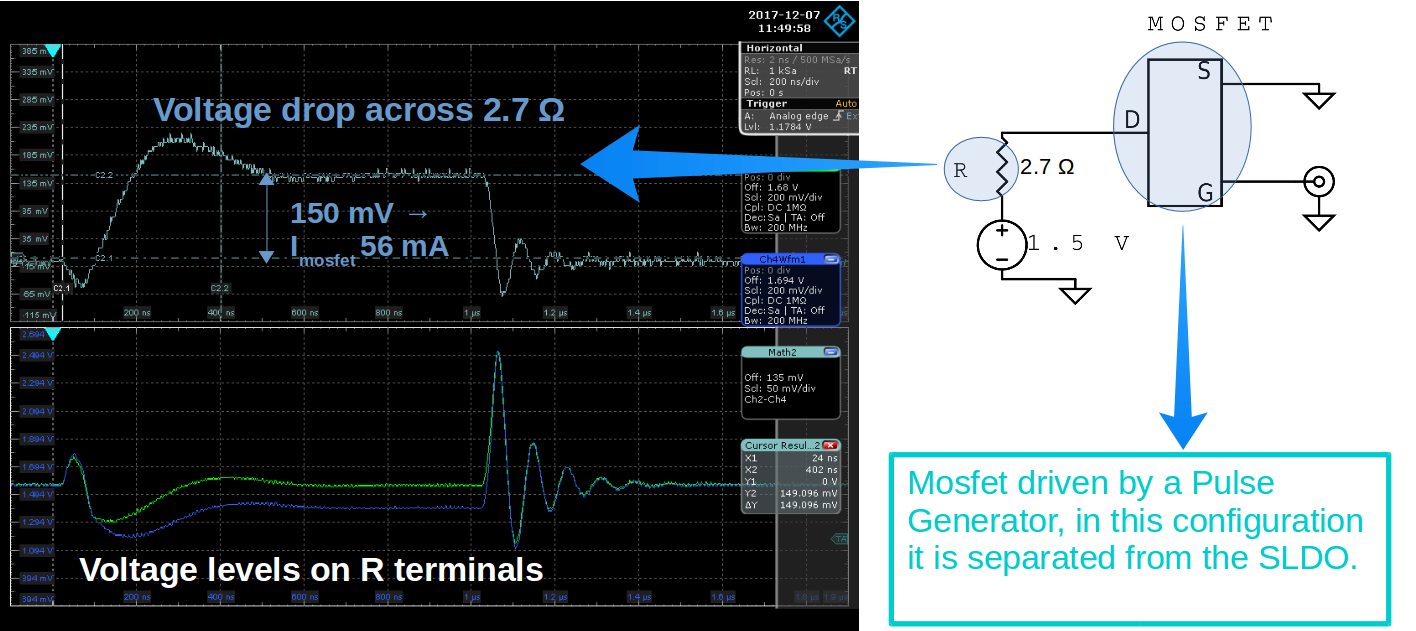
\includegraphics[width=\linewidth]{Immagini/MosfetBehaviourbis}
\caption{Schermata dell'oscilloscopio (a sinistra) che mostra l'andamento della tensione ai capi del resistore da $2.7\Ohm$ in funzione del tempo; a destra è invece riportato lo schema del circuito di prova del mosfet.}
\label{MosfetBehaviour}
\end{figure}

Per esaminare il comportamento del mosfet in risposta all'impulso sul Gate, si è realizzato un allestimento di test specifico, mostrato nella parte a destra della Fig.~\ref{MosfetBehaviour}: il Drain del mosfet è stato disconnesso dal resto del circuito della scheda di test e connesso ad una batteria esterna da $\sim 1.5\V$, che emula $\mathrm{V_{out}}$ senza per\`o alterare i profili temporali, con in serie una resistenza di $2.7\Ohm$, utilizzata per misurare le correnti che sorrono nel mosfet. 
%Per esaminare il comportamento del mosfet in risposta all'impulso mandato sul Gate, si è proceduto ad isolare questa parte del circuito dal resto della scheda di test, connettendo al Drain una resistenza in serie ad una batteria stilo, al posto della connessione con il $\mathrm{V_{out}}$ dello ShuntLDO.
%La batteria ricopre il ruolo di $\mathrm{V_{out}}$, mentre la resistenza è necessaria alla misura delle correnti che scorrono nel mosfet ed ha un valore di 2.7 $\Omega$. 

La Fig.~\ref{MosfetBehaviour} a sinistra, mostra la caduta di tensione ai capi della resistenza in serie alla batteria: le oscillazioni già osservate con lo ShuntLDO connesso e presenti in corrispondenza dello spegnimento del mosfet, sono evidenti anche con questo allestimento.
Esse sono, dunque, generate dal mosfet stesso nel momento in cui il canale, che collega Drain e Source, si interrompe e non dipendono da $\mathrm{V_{out}}$.
Inoltre, il fronte di salita della corrente (ovvero della differenza di potenziale ai capi della resistenza) ha una durata di $\sim 100 \ns$, maggiore dei $40\ns$ di salita dell'impulso di gate impostati sul generatore. I test dinamici, quindi, devono tener conto di questa limitazione intrinseca del mosfet utilizzato. Esaminando i data-sheet di questo componente di potenza (ZXMN20B28K~\cite{MOSFET}) si può verificare che il suo tempo di ``accensione'' (\textit{Turn-on rise time}) è $\sim 80 \ns$ e che \`e inoltre caratterizzato da capacità in ingresso non piccola, pari a $\sim 360\pF$.
\begin{figure}
\centering
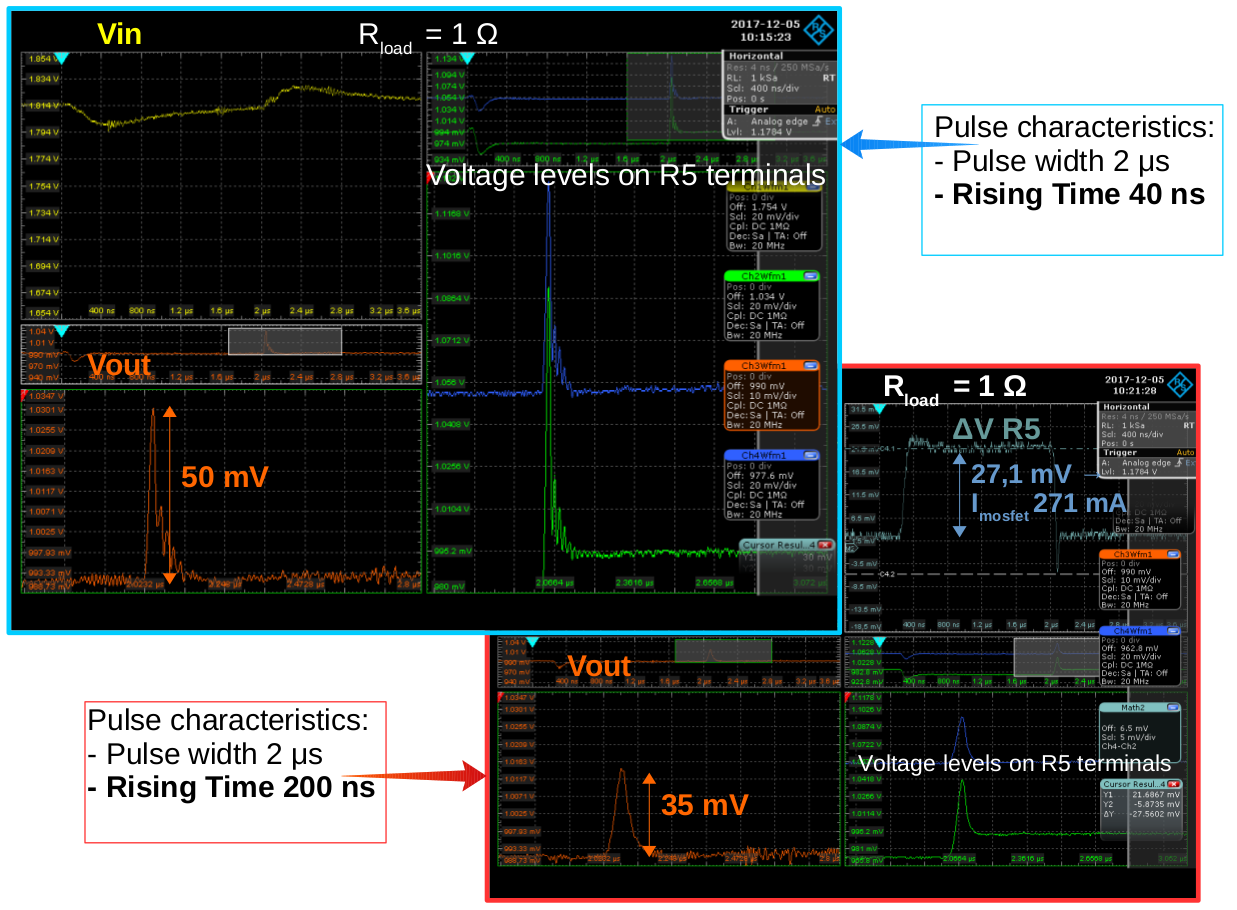
\includegraphics[width=\linewidth]{Immagini/RiseTime}
\caption{Andamento di $\mathrm{V_{out}}$ e delle tensioni ai capi di `R5' per impulsi di corrente addizionale con diverso tempo di commutazione: $40\ns$ (a sinistra in alto), $200\ns$ (in basso a destra). Tutte le osservabili migliorano nel comportamento con impulsi pi\`u lenti.}
\label{RiseTime}
\end{figure}

La risposta dello ShuntLDO per segnali dell'impulsatore più veloci della risposta del mosfet è quindi mascherata da quest'ultimo, motivo per cui si è deciso di utilizzare, per le misure successive, un tempo di salita del segnale del generatore di impulsi non inferiore a $200\ns$. Questa problematica non \`e stata osservata con il mosfet presente sulla scheda di test dello ShuntLDO a $0.5\A$ dato che, grazie al minore dimensionamento in corrente, \`e stato utilizzato un mosfet con prestazioni temporali migliori.

La Fig.~\ref{RiseTime} mostra il miglioramento fra la configurazione con i tempi di commutazione del generatore di impulsi a $40 \ns$ e quella con $200 \ns$. Con quest'ultima configurazione è possibile verificare la risposta dello ShuntLDO ad una variazione di carico più lenta, ma non inquinata dalle caratterisitiche del mosfet. Lo studio per domini temporali di commutazione pi\`u brevi di $\sim 200\ns$ \`e rimandato ad uno studio futuro perch\`e richiede un allestimento di prova migliorato. Si pu\`o comunque precisare che questa scala temporale \`e confrontabile con il confine tra il regime di intervento dei condensatori di disaccoppiamento e quello in cui le fluttuazioni di carico sono gestite dallo ShuntLDO~\cite{saramarconi}.
 
%In figura \ref{RiseTime} è visibile come la situazione precedente, in cui l'impulso ha un tempo di salita di 40 ns, migliora visibilmente passando a 200 ns, in questo modo quello che viene simulato all'uscita dello ShuntLDO è un variazione di carico più lenta ma il cui comportamento è affetto in modo minore dalle caratteristiche del mosfet. 

\subsubsection{Caratterizzazione con variazioni di carico veloci}

Di seguito sono riportate le misure di caratterizzazione della tensione di ingresso, $\mathrm{V_{in}}$, e di uscita, $\mathrm{V_{out}}$, per tre differenti valori di $\mathrm{R_{load}}$ e al variare dell'entit\`a dell'impulso di $\mathrm{I_{mosfet}}$.
I valori di $\mathrm{R_{load}}$ scelti sono di $1\Ohm$, $2.1\Ohm$ e $4\Ohm$ e, dato che $\mathrm{V_{out}=1\V}$, questi corrispondono rispettivamente a $1\A$, $0.475\A$ e $0.250\A$ in termini di correnti statiche $\mathrm{I_{load}}$,.
%Oltre alla misura delle variazioni in ampiezza di $\mathrm{V_{in}}$ e $\mathrm{V_{out}}$ sono stati misurati anche i tempi di  recupero delle stesse.

Lo ShuntLDO è alimentato in corrente con $\Iin = 1.5\A$. Nel momento in cui $\mathrm{I_{load}+I_{mosfet}}$ raggiunge valori vicini o addirittura superiori  a $\Iin$, si ha un crollo di $\Vin$ e di $\mathrm{V_{out}}$ poiché si sta chiedendo allo ShuntLDO di fornire una corrente superiore a quella a sua disposizione.
Per ciascun valore di $\mathrm{R_{load}}$, dunque, è stata fatta variare la corrente assorbita dal mosfet $\mathrm{I_{mosfet}}$ fino ad arrivare a valori critici misurando le variazioni di $\mathrm{V_{out}}$ e $\mathrm{V_{in}}$. 

Le misure eseguite prendono evidentemente in considerazione anche situazioni in cui la variazione di corrente su $\VDD$ supera di molto il $20-25\%$ che corrisponde alla stima delle  variazione massime di carico che devono essere gestite dallo ShuntLDO durante la normale attivit\`a del ROC~\cite{saramarconi}. Le misure in cui la variazione del carico è il doppio del valore statico possono per\`o aver luogo al momento dell'accensione del ROC. %, le cui variazioni di consumo in regime di lavoro, di norma, non superano i 500 mA.(controllare) 

Come detto in precedenza, gli impulsi utilizzati presentano una durata che consente di differenziare tra gli effetti dovuti al fronte di salita e quelli prodotti dal fronte di discesa. 
Facendo riferimento alla Fig.~\ref{VoutUnd}, si possono vedere, in valore assoluto,

L'entit\`a della riduzione di $\VDD$ \`e visibile in~Fig.~\ref{VoutUnd} per i tre valori del carico statico: in funzione della corrente totale $\mathrm{I_{tot} = I_{load}+I_{mosfet}}$ a sinistra; in funzione di $\mathrm{I_{mosfet}}$ a destra. 
%I primi risultati riportano gli undershoot della tensione di uscita a cui è applicato il carico, riferendosi ai grafici in Fig.~\ref{VoutUnd} sono riportati i valori assoluti di tali variazioni in funzione della corrente che scorre nel mosfet (sinistra) e della corrente totale (destra), la corrente totale è somma di quella assorbita dal carico e dal mosfet. 
\begin{figure}
\centering
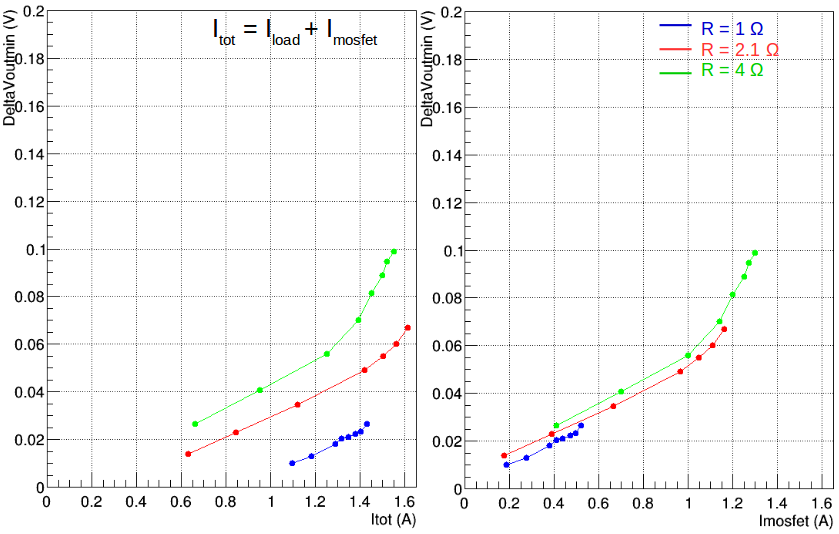
\includegraphics[width=0.9\linewidth]{Immagini/VoutUnd}
\caption{Riduzione di $\mathrm{V_{out}}$ in funzione di $\mathrm{I_{tot} = I_{load}+I_{mosfet}}$ (a sinistra) e di $\mathrm{I_{mosfet}}$ (a destra) per tre valori del carico statico: $1\Ohm$-$1\A$ (blu), $2.1\Ohm$-$0.475\A$ (rosso) e $4\Ohm$-$0.250\A$ (verde).}
\label{VoutUnd}
\end{figure}
Il grafico a destra mostra una caratteristica importante del circuito di ShuntLDO, ossia che la variazione di $\mathrm{V_{out}}$ dovuta a variazioni del carico, in questo caso l'improvvisa ``richiesta'' di corrente da parte del mosfet pilotato dall'impulsatore, dipende solo da quest'ultima e non anche dall'entit\`a del carico statico a cui si va ad aggiungere. Infatti le tre curve riportate sono essenzialmente sovrapposte tenendo conto delle incertezze sulla misura.
Si osserva inoltre che, nell'ambito di variazioni di corrente realistiche per il normale funzionamento del ROC, le variazioni di $\mathrm{V_{out}}$ sono relativamente piccole di $\mathrm{V_{out}}$ e assolutamente entro le specifiche richieste. Ad esempio, con $\mathrm{I_{mosfet}= 0.4\A}$, $\mathrm{\Delta V_{out} \simeq 20\mV}$.

%
% ------------------------------------ Sono arrivato qui
%

\begin{figure}
\centering
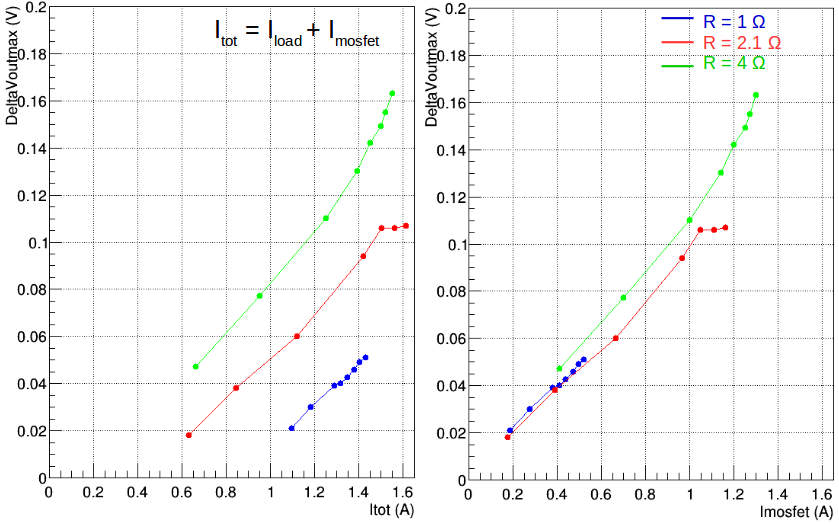
\includegraphics[width=0.9\linewidth]{Immagini/VoutOver}
\caption{Grafici che riportano l'entità dell'overshoot del $\mathrm{V_{out}}$ in funzione della corrente totale, grafico di sinistra, e della corrente del mosfet, grafico di destra.}
\label{VoutOver}
\end{figure}
%Come si può vedere dal grafico di destra, le tre curve seguono lo stesso andamento, dato che vi è una relazione fra la variazione di $\mathrm{V_{out}}$ e $\mathrm{I_{mosfet}}$, indipendente dal valore della resistenza.

Un comportamento analogo si riscontra dai grafici di Fig.~\ref{VoutOver}, dove è riportata l'entità delle variazioni di $\mathrm{V_{out}}$ a seguito dello spegnimento del mosfet, cioè l'effetto che si ha sul fronte di discesa dell'impulso. 
%Nell'esaminare questi andamenti va ricordato che la corrente in ingresso al circuito è 1.5 A, quindi punti per i quali si ha una $\mathrm{I_{tot}}$ vicina o superiore a questo valore sono ottenuti in una situazione in cui lo ShuntLDO è impossibilitato a compiere il suo lavoro. 
%Ricordiamo che la corrente che passa in $R_3$ è un millesimo di quella che scorre nel ramo in cui si hanno carico e shunt.

Come per il $\mathrm{V_{out}}$ è stato misurato l'undershoot e l'overshoot della tensione in ingresso $\mathrm{V_{in}}$: i grafici dei primi sono riportati in Fig.~\ref{VinUnd}, quelli dei secondi in Fig.~\ref{VinOver}. 
\begin{figure}
\centering
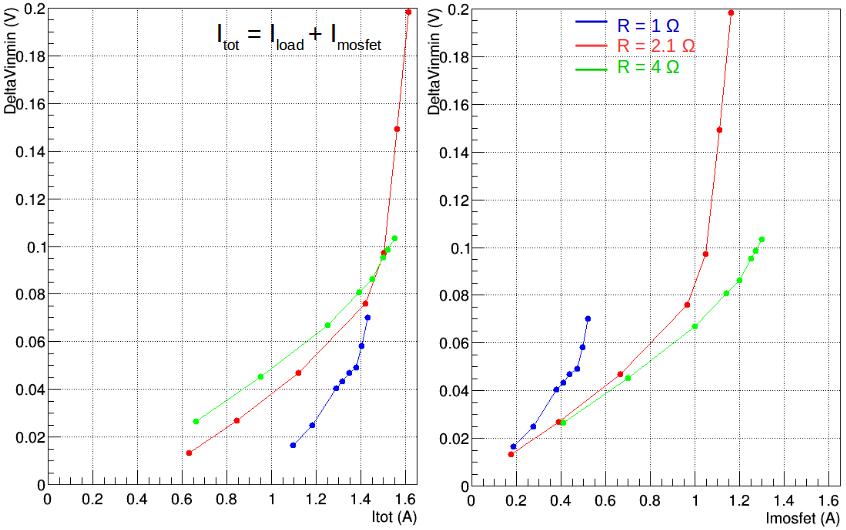
\includegraphics[width=0.9\linewidth]{Immagini/VinUnd}
\caption{Grafici che riportano l'entità dell'undershoot del $\mathrm{V_{in}}$ in funzione della corrente totale, grafico di sinistra, e della corrente del mosfet, grafico di destra.}
\label{VinUnd}
\end{figure}
\begin{figure}
\centering
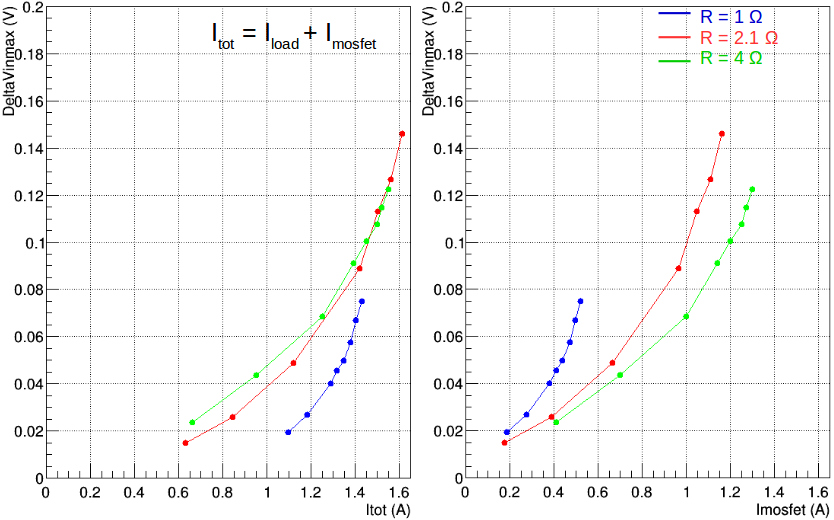
\includegraphics[width=0.9\linewidth]{Immagini/VinOver}
\caption{Grafici che riportano l'entità dell'undershoot del $\mathrm{V_{in}}$ in funzione della corrente totale, grafico di sinistra, e della corrente del mosfet, grafico di destra.}
\label{VinOver}
\end{figure}
In entrambi i casi la variazione della tensione in ingresso dipende sia dalla variazione di corrente $\mathrm{I_{mosfet}}$ che dalla corrente fissa $\mathrm{I_{load}}$. 
Si è osservato inoltre che, per valori elevati di $\mathrm{I_{mosfet}}$, la tensione in ingresso inizia ad oscillare, con periodi di qualche $\mu$s.
Questo comportamento è dovuto al generatore utilizzato per questi test in cui l'alimentazione in corrente è ottenuta utilizzando un generatore di tensione limitato in corrente. 
Infatti, nel momento in cui si ha una variazione di carico molto veloce, che provoca un abbassamento di $\mathrm{V_{out}}$, si ha una piccola ripercussione sulla tensione di ingresso: dato che il generatore è di tensione, limitato in corrente, per tenere costante $\mathrm{I_{in}}$ avrà un abbassamento di tensione, ma con tempi più lunghi rispetto a quelli con cui lo ShuntLDO riesce a riequilibrare $\mathrm{V_{out}}$.
Il comportamento oscillatorio di $\mathrm{V_{in}}$, che compare quando $\mathrm{I_{tot}}$ è intorno al valore massimo, $\mathrm{I_{in}}$, ha permesso di constatare come fluttuazioni della tensione in ingresso non influiscano comunque sulla tensione generata dal regolatore.

Una prima interessante osservazione, visibile in Fig.~\ref{DipVoutVin}, \`e relativa ai tempi di recupero di $\mathrm{V_{in}}$ e $\mathrm{V_{out}}$ in seguito alla variazione di carico. Questi differiscono notevolmente: il primo è dell'ordine dei $\us$, e dipendente dal valore di $\mathrm{I_{mosfet}}$, il secondo, più veloce, ha durata di circa $300\ns$ indipendentemente dal valore di $\mathrm{I_{mosfet}}$. Il comportamento di $\mathrm{V_{in}}$, a monte del circuito di ShuntLDO, è imputabile alla velocità con cui il generatore esterno reagisce al transiente seppur limitato in ampiezza. Il comportamento di $\mathrm{V_{out}}$, invece, dimostra la velocità di recupero dello ShuntLDO stesso, caratteristica fondamentale del suo funzionamento.
\begin{figure}
  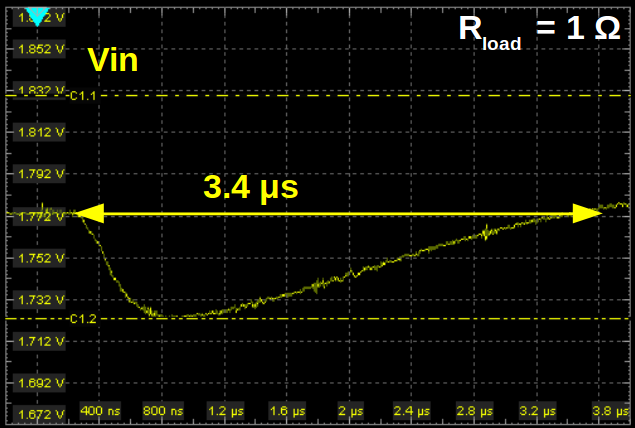
\includegraphics[width=.48\linewidth]{Immagini/zoomDipendenzaVoutdaVin1}
  \hfill
  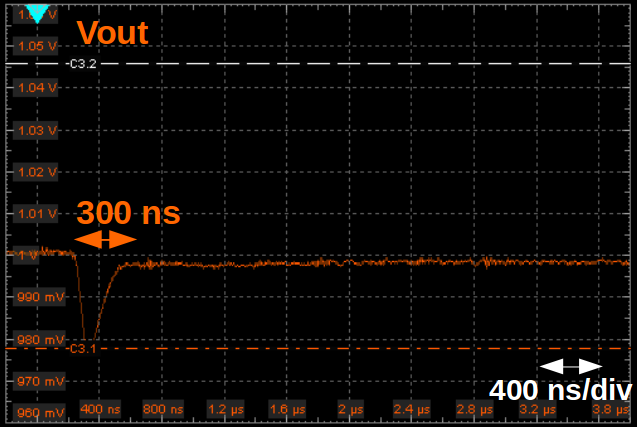
\includegraphics[width=.48\linewidth]{Immagini/zoomDipendenzaVoutdaVin2}
\caption{Differenze nei tempi di recupero tra $\mathrm{V_{in}}$ (a sinistra, giallo), e $\mathrm{V_{out}}$ (a destra, arancione).}
\label{DipVoutVin}
\end{figure}


%Questo può essere visto utilizzando l'oscilloscopio: in Fig.\ref{DipVoutVin} è mostrata una schermata dell'oscilloscopio in cui è riportato, in giallo, l'andamento di $\mathrm{V_{in}}$ in funzione del tempo, e, in arancione, la tensione di $\mathrm{V_{out}}$.
%Si nota che le scale di tempo di recupero sono differenti, i.e. alcuni $\mu$s per $\mathrm{V_{in}}$ e circa $300 \ns$ per $\mathrm{V_{out}}$.

%\begin{figure}
%\centering
%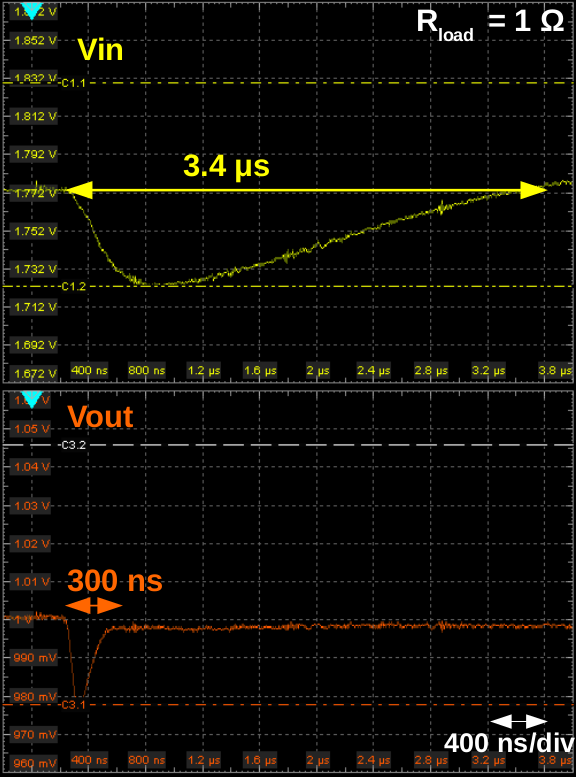
\includegraphics[scale=.35]{Immagini/DipendenzaVoutdaVin}
%\caption{Differenze nei tempi di recupero tra $\mathrm{V_{out}}$, in giallo, e $\mathrm{V_{out}}$, in arancione.}
%\label{DipVoutVin}
%\end{figure}

\subsubsection{Serie di due ShuntLDO}

Dato che eventuali oscillazioni della tensione in ingresso causerebbero oscillazioni di tensione in tutta la catena di moduli, è importante che queste non si ripercuotano sul $\mathrm{V_{out}}$. 
Per verificare questo aspetto si è misurato con l'oscilloscopio la tensione di uscita di uno ShuntLDO messo in serie ad un secondo a cui è applicato un carico variabile, tramite l'utilizzo del mosfet, come già visto nelle misure precedenti.
In Fig.~\ref{SLDOserie} sono affiancati uno schema del setup (sinistra) e la foto dei due ShuntLDO in serie (destra). 
Il serie di due ShuntLDO, entrambi con un carico statico di $4 \Ohm$, è alimentato con una corrente in ingresso di $1.5 \A$ e sul secondo ShuntLDO è collegato l'impulsatore che regola l'assorbimento di corrente  da parte del mosfet. 
Acquisendo con l'oscilloscopio la tensione di $\mathrm{V_{out}}$ di entrambi e il $\mathrm{V_{in}}$ del primo ShuntLDO della catena (quello con il solo carico statico) è stato possibile verificare come le fluttuazioni di tensione non influenzino la generazione della tensione di $\mathrm{V_{out}}$.
\begin{figure}[h!]
\centering
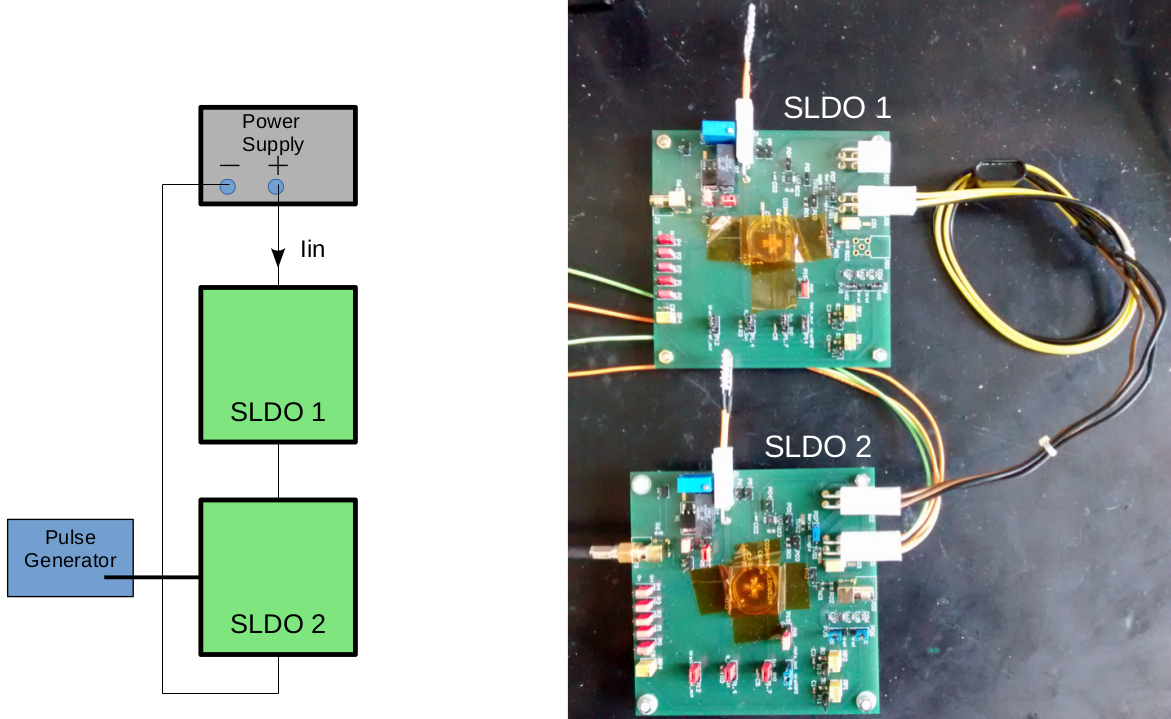
\includegraphics[scale=.30]{Immagini/SLDOserie}
\caption{Sulla destra foto dei due ShuntLDO in serie di cui a sinistra è riportato uno schema delle connessioni con generatore e impulsatore.}
\label{SLDOserie}
\end{figure}
In particolare in Fig.~\ref{ScreenSerie} si vede che, nonostante il secondo ShuntLDO sia in una situazione estrema, la generazione di $\mathrm{V_{out}}$ da parte del primo non ha ripercussioni. 
Il campionamento dei segnali mostrati, acquisiti con l'oscilloscopio, è stato ottenuto con una $\mathrm{I_{mosfet}}$ di $1.2 \A$, corrispondenti ad una $\mathrm{I_{tot}}$ di circa $1.45 \A$, quindi molto vicino al limite di $1.5 \A$. 
\begin{figure}[h!]
\centering
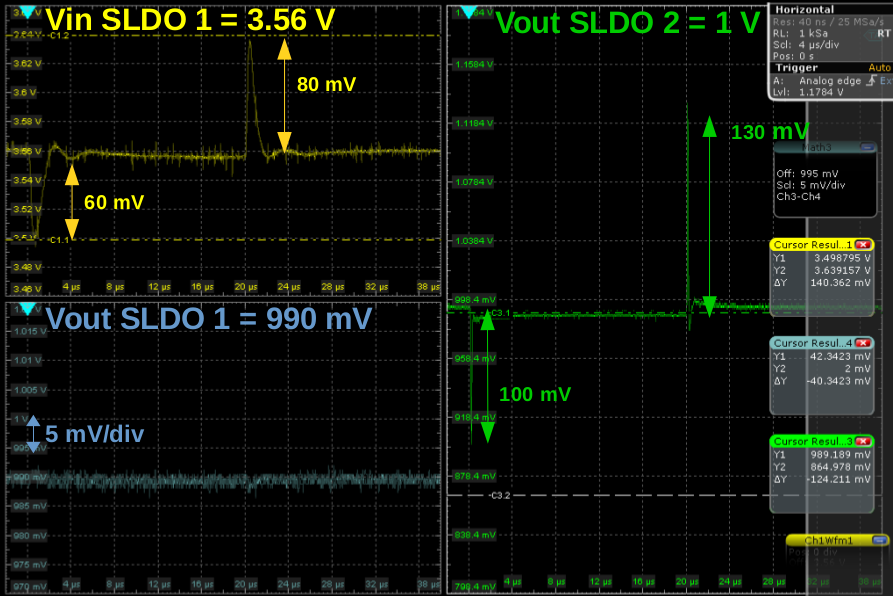
\includegraphics[scale=.32]{Immagini/ScreenSerie}
\caption{Schermata dell'oscilloscopio in cui è riportata in giallo la tensione in ingresso al primo ShuntLDO della catena,  in celeste la tensione di $\mathrm{V_{out}}$ sempre dello ShuntLDO1 e in verde la tensione di $\mathrm{V_{out}}$ dello ShuntLDO2 su cui è applicato il carico dinamico. Le fluttuazioni in tensione originate dalla variazione di carico sullo ShuntLDO2 si ripercuotono sul $\mathrm{V_{in}}$ dello ShuntLDO1 (giallo) ma non sulla tensione da esso generata (celeste).}
\label{ScreenSerie}
\end{figure}
In verde è riportato l'andamento di $\mathrm{V_{out}}$ del secondo ShuntLDO, che mostra importanti undershoot e overshoot, i quali, a loro volta e come visto in precedenza, causano fluttuazioni della tensione in ingresso. 
La tensione di ingresso dello ShuntLDO2 corrisponde alla terra della scheda di test su cui si trova lo ShuntLDO1.
Le visibili fluttuazioni di questa, quindi, si ripercuotono su ShuntLDO2.
Nonostante ciò, come risultato importante, si può notare che $\mathrm{V_{out}}$ del primo ShuntLDO è indipendente da queste.
